\documentclass[../report.tex]{subfiles}
%\graphicspath{{\subfix{../img/}}}

\begin{document}
\subsection{Time management}
We aimed to include everyone in all areas of the project development. This meant
we insured that everyone got the opportunity to be involved, with a task
fitting to there knowledge level.

We began with creating a general time plan for the whole semester project
progress.
\begin{figure}[H]
    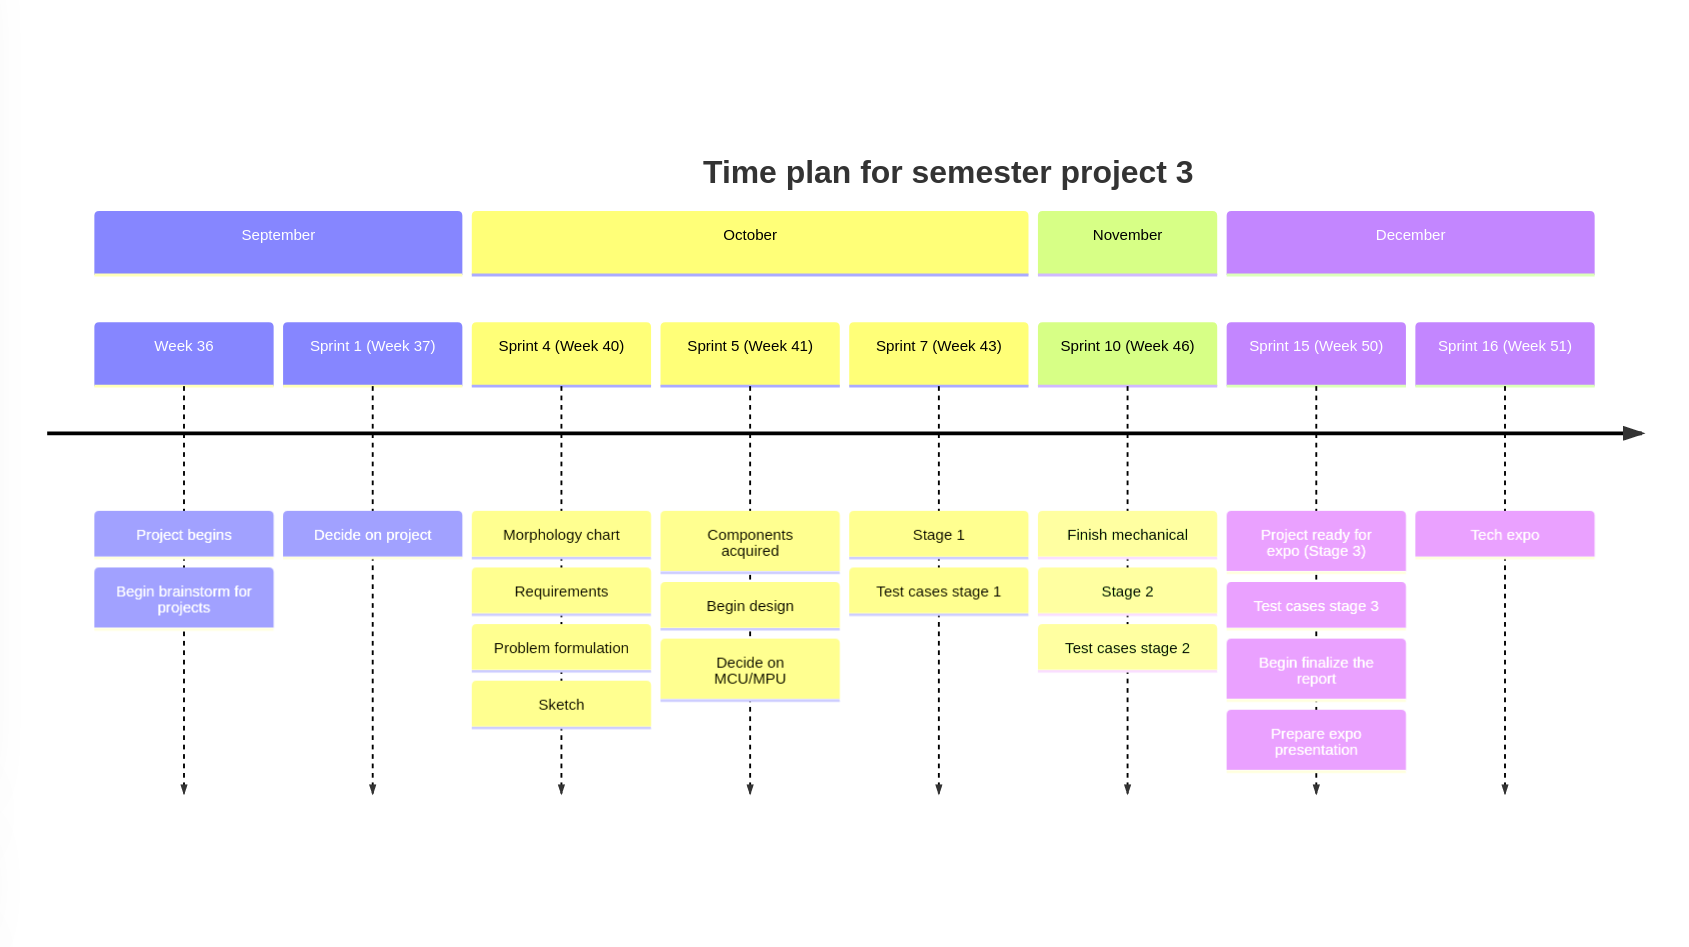
\includegraphics[width=\textwidth]{Management/timeplan.png}
    \caption{Initial time plan}
\end{figure}

\subsection{Task management}

For the semester period the Scrum agile management framework was adopted and customized to fit our project
and teams needs. We chose specifically this model due to the agile planing it introduces, and gradual
learning curve. We defined a sprint to be 7 days, from friday to friday with an estimate of 8 hours of
workload per team member. We categorized each task according to the time estimated to complete it
using these tags:

\begin{itemize}
    \item Sønderborg - 0.5 hours
    \item Kiel - 1 hours
    \item Valencia - 2 hours
    \item Budapest - 4 hours
    \item Hamburg -  6 hours
\end{itemize}

We chose our home cities and sorted them by size (one member joined later - hence, just 5) to make it more simple to use
in conversations and to give a better visual idea of the task size. We decided
that the time limited on a task should be 6 hours. If a task would require more
time then it should be split into multiple tasks. This was to ensure that it
was possible to see if the task was possible to achieve before investing more
time into it.

Throughout the semester period stand-up meetings according to the scrum model
were conducted every Wednesday. This was to touch base and catch any potential
problems. The meeting was written down usually in the following format:

\textbf{Week 49 (Sprint 10)}
\begin{table}[H]
    \begin{center}
        \begin{tabularx}{\linewidth}{L|L|L|L}
            
            \textbf{Name} & \textbf{What did I work on?} & \textbf{What am I working on? }& \textbf{What issues are blocking me?} \\
            \hline
            \textbf{Henrik} & consulted teacher about the sensors: wheatstone bridge, setup, went to the labs & try to implement it, constant source, LT spice, test weight sensor &  \\
            \hline
            \textbf{Laura} & model of the IR sensor, went to the lab with Henrik & develop further the amplifier  & \\
            \hline
            \textbf{Boti} & writing code for the IR sensor:analog sensor & test to differentiate different materials for the sensor & no printers available\\
            \hline
            \textbf{Felix} & report management task, physical assembly of the mast, cut the guide rodes & mast assembly & printers \\
            \hline
            \textbf{Arthur} & researching how to build the pcb of the drivers & design motor pcb & \\
            \hline
            \textbf{Casper} & created test cases & continue with the same task & time problems
        \end{tabularx}
    \end{center}
    \caption{Sample of a weekly stand-up meeting}
\end{table}

During the project period, we observed that the Scrum model functioned
effectively when the workload was manageable. However, given the intensiveness
of the last phase of the project, the workload for upcoming tasks was
anticipated to be too substantial for Scrum to provide optimal benefits. As a
result, we decided to retain the Kanban board for task management. Instead of
having one person create and assign tasks, each individual team member was
empowered to take ownership of task creation and assignment.

\end{document}